% ===========================================================================
%  INFORME TÉCNICO — PREDICCIÓN DEL PESO FINAL DE POLLOS DE ENGORDE
%  Caso práctico de Ciencia de Datos aplicada a la avicultura (Ecuador)
%
%  Compilación recomendada (2 pasadas para índice y referencias cruzadas):
%     pdflatex informe_latex.txt
%     pdflatex informe_latex.txt
%
%  Requiere las figuras en la subcarpeta ./figuras/ (incluidas en el repo).
% ===========================================================================
\documentclass[11pt,a4paper]{article}

\usepackage[utf8]{inputenc}
\usepackage[T1]{fontenc}
\usepackage[spanish,es-tabla]{babel}
\usepackage{lmodern}
\usepackage[margin=2.4cm]{geometry}
\usepackage{graphicx}
\usepackage{booktabs}
\usepackage{array}
\usepackage{longtable}
\usepackage{amsmath}
\usepackage{amssymb}
\usepackage{siunitx}
\usepackage{xcolor}
\usepackage{colortbl}
\usepackage{caption}
\usepackage{subcaption}
\usepackage{float}
\usepackage{enumitem}
\usepackage{fancyhdr}
\usepackage{titlesec}
\usepackage[hidelinks,colorlinks=true,linkcolor=azulcorp,urlcolor=azulcorp,citecolor=azulcorp]{hyperref}

% --- Paleta corporativa sobria ---
\definecolor{azulcorp}{RGB}{31,78,121}
\definecolor{grisclaro}{RGB}{242,242,242}
\definecolor{verdeok}{RGB}{0,128,96}

\graphicspath{{figuras/}}

% --- Encabezados / pies ---
\pagestyle{fancy}
\fancyhf{}
\lhead{\small\textcolor{azulcorp}{Predicción de peso final — Pollos de engorde}}
\rhead{\small\thepage}
\renewcommand{\headrulewidth}{0.4pt}
\renewcommand{\arraystretch}{1.18}

% --- Estilos de sección ---
\titleformat{\section}{\Large\bfseries\color{azulcorp}}{\thesection.}{0.6em}{}
\titleformat{\subsection}{\large\bfseries\color{azulcorp!85}}{\thesubsection.}{0.5em}{}

\sisetup{group-separator={\,},output-decimal-marker={,}}

% --- Cajas de hallazgo ---
\newcommand{\hallazgo}[1]{%
  \par\medskip\noindent\colorbox{grisclaro}{%
  \begin{minipage}{0.985\linewidth}\small\vspace{2pt}\textbf{\textcolor{azulcorp}{Hallazgo.}}\ #1\vspace{2pt}\end{minipage}}\par\medskip}

\begin{document}

% =========================================================================
% PORTADA
% =========================================================================
\begin{titlepage}
\centering
\vspace*{1.2cm}
{\color{azulcorp}\rule{\linewidth}{1.4pt}}\\[0.5cm]
{\Huge\bfseries\color{azulcorp} Predicción del Peso Final\\[0.2cm] de Pollos de Engorde\par}
\vspace{0.35cm}
{\Large Un pipeline reproducible de Ciencia de Datos para la toma de decisiones en planta avícola\par}
\vspace{0.25cm}
{\color{azulcorp}\rule{\linewidth}{1.4pt}}\\[1.4cm]

{\large\itshape Informe técnico del caso práctico\par}
\vspace{0.4cm}
{\large De la limpieza del dato a la conclusión capitalizable\par}
\vspace{2.2cm}

\begin{minipage}{0.85\textwidth}\centering\small
\textbf{Objetivo.} Construir y validar un modelo capaz de \emph{predecir el peso final} de un lote de
pollos de engorde a partir de variables de manejo, ambiente y genética, y traducir el modelo en
\textbf{recomendaciones operativas auditables}: qué línea genética conviene, qué variables
gobiernan el engorde, cuánto alimento se consume y dónde está el dinero.
\end{minipage}

\vfill
{\small Trabajo desarrollado íntegramente en Python (\textit{scikit-learn}, \textit{statsmodels},
\textit{XGBoost}, \textit{LightGBM}). Cuaderno reproducible con semilla fija (\texttt{random\_state = 42}).\par}
\vspace{0.3cm}
{\small\textbf{Ecuador — 2026}\par}
\end{titlepage}

\tableofcontents
\thispagestyle{empty}
\clearpage

% =========================================================================
% 1. RESUMEN EJECUTIVO
% =========================================================================
\section{Resumen ejecutivo}

Se analizó un conjunto de \num{1000} registros de lotes de pollos de engorde con \num{11} variables,
con el fin de predecir el \textbf{peso final (\si{\gram})} y extraer conclusiones útiles para la
operación. El trabajo siguió un pipeline completo y reproducible: comprensión del dato, limpieza,
análisis exploratorio (EDA), selección de variables con control estricto de \emph{fuga de información},
comparación de once modelos —estadísticos y de \emph{machine learning}— y análisis de importancia con
lectura de negocio.

\medskip
Los resultados principales son:

\begin{itemize}[leftmargin=1.4em,itemsep=3pt]
  \item \textbf{El crecimiento es esencialmente lineal en la ventana de cría (1--42 días).} La edad
        explica por sí sola el \SI{98.1}{\percent} de la varianza del peso final; añadir el consumo de
        alimento, el sexo, la línea genética y el ambiente aporta mejoras marginales.
  \item \textbf{Modelo campeón: regresión Lasso} (lineal regularizada), con
        \textbf{RMSE de \SI{83.08}{\gram}}, \textbf{MAE de \SI{64.58}{\gram}},
        \textbf{$R^2 = 0{,}9921$} y \textbf{MAPE de \SI{5.82}{\percent}} sobre datos de prueba no vistos.
        Los modelos de árboles (XGBoost, LightGBM, Random Forest) \emph{no} superaron a la familia
        lineal: se eligió el modelo más simple, interpretable y desplegable (principio de parsimonia).
  \item \textbf{El sexo pesa más que la genética.} Controlando edad y línea, los machos pesan en
        promedio \SI{+126.4}{\gram} más que las hembras (IC\,95\%: \numrange{113.2}{139.7}).
  \item \textbf{Ranking de líneas (efecto ajustado por edad y sexo):} \textbf{Cobb 500} encabeza con
        \SI{+44.3}{\gram} (IC\,95\%: \numrange{28.1}{60.5}) sobre Arbor Acres, seguida de
        \textbf{Ross 308} con \SI{+25.2}{\gram} (IC\,95\%: \numrange{9.1}{41.4}). Ambos efectos son
        estadísticamente significativos y coinciden con la literatura para clima tropical.
  \item \textbf{Impacto económico.} A precio de mercado de referencia (\SI{1.65}{USD\per\kilo} en pie),
        migrar un lote de \num{10000} aves a Cobb 500 frente a Arbor Acres añade del orden de
        \textbf{\SI{1481}{USD} por lote} en ingreso bruto solo por mayor peso.
  \item \textbf{Las variables ambientales (temperatura, humedad, mortalidad) aparecen como ruido} en
        este dataset (información mutua nula con el objetivo). Es un \emph{hallazgo de calidad del dato},
        no una verdad biológica: la literatura sí documenta su efecto. Se recomienda mejorar la
        sensórica y el registro para capitalizar esa señal.
\end{itemize}

% =========================================================================
% 2. DATOS Y METODOLOGÍA
% =========================================================================
\section{Datos y metodología}

\subsection{El conjunto de datos}
La base contiene \num{1000} observaciones (lotes) y \num{11} columnas. La variable objetivo es
\texttt{Peso\_Final\_g}. El resto se agrupa en cuatro bloques: \emph{tiempo} (\texttt{Edad\_Dias}),
\emph{manejo/ambiente} (\texttt{Consumo\_Alimento\_g\_dia}, \texttt{Temperatura\_C},
\texttt{Humedad\_\%}, \texttt{Densidad\_Aves\_m2}, \texttt{Mortalidad\_\%}), \emph{biología}
(\texttt{Sexo}, \texttt{Linea\_Genetica}, \texttt{Peso\_Inicial\_g}) e \emph{identificación}
(\texttt{ID\_Lote}).

\subsection{Hoja de ruta del análisis}
El pipeline implementado en el cuaderno \texttt{pipeline\_pollos.ipynb} cubre, en orden, las siete etapas
del encargo: (1) conocer el dato, (2) preparar el terreno —limpieza, faltantes, \emph{outliers},
ingeniería de variables—, (3) EDA, (4) selección de variables, (5) modelado, (6) comparación de
métricas y (7) importancia de variables y recomendaciones. Todo el flujo es reproducible con semilla
fija y los artefactos (figuras y tablas) se persisten automáticamente en \texttt{outputs/}.

% =========================================================================
% 3. PREPARACIÓN Y LIMPIEZA
% =========================================================================
\section{Comprensión y limpieza del dato}

\subsection{Calidad de los datos}
La auditoría de calidad fue, en buena medida, una buena noticia: \textbf{no hay valores nulos, ni
duplicados, ni centinelas} (códigos del tipo $-1$/\num{999} usados para marcar ausencias). El único
``\num{999}'' presente corresponde a un \texttt{ID\_Lote} legítimo dentro de una secuencia
\numrange{1}{1000}. Las clases categóricas están balanceadas: sexo $\approx$ 50/50 y las tres líneas
genéticas con $\approx$ 330 lotes cada una. La Tabla~\ref{tab:calidad} resume el diagnóstico.

\begin{table}[H]
\centering
\caption{Diagnóstico de calidad y rango de las variables.}
\label{tab:calidad}
\small
\begin{tabular}{l c c c S[table-format=4.2] S[table-format=4.2]}
\toprule
\textbf{Variable} & \textbf{Tipo} & \textbf{Nulos} & \textbf{Únicos} & {\textbf{Mín.}} & {\textbf{Máx.}}\\
\midrule
Edad\_Dias              & entero  & 0 & 42  & 1.00   & 42.00\\
Consumo\_Alimento\_g\_dia & decimal & 0 & 771 & 20.00  & 231.10\\
Temperatura\_C          & decimal & 0 & 141 & 20.00  & 34.00\\
Humedad\_\%             & decimal & 0 & 376 & 45.00  & 85.00\\
Densidad\_Aves\_m2      & decimal & 0 & 101 & 8.00   & 18.00\\
Mortalidad\_\%          & decimal & 0 & 406 & 0.00   & 6.48\\
Peso\_Inicial\_g        & decimal & 0 & 101 & 38.00  & 48.00\\
Peso\_Final\_g (objetivo) & decimal & 0 & 975 & 135.00 & 3596.30\\
\bottomrule
\end{tabular}
\end{table}

\subsection{Faltantes y valores atípicos}
Dado que no existen faltantes, no fue necesaria imputación; aun así, el preprocesamiento incluye
imputación por mediana (numéricas) y moda (categóricas) como \emph{salvaguarda} para datos futuros en
producción. En cuanto a \emph{outliers}, el análisis sobre la curva de crecimiento mostró apenas dos
puntos con $|z| > 3$ y ninguno con $|z| > 4$. \textbf{No se eliminó ni se winsorizó ningún registro}:
los puntos extremos siguen el patrón general (aves muy jóvenes o muy próximas a faena) y eliminarlos
sesgaría el modelo.

\hallazgo{El dato presenta un \textbf{artefacto de origen sintético}: a día~1 el peso medio ronda los
\SI{373}{\gram}, biológicamente imposible para un pollito BB (que pesa \SIrange{40}{45}{\gram}, coherente
con \texttt{Peso\_Inicial\_g}). La recta de crecimiento tiene un intercepto no físico ($\approx$\,\SI{260}{\gram}).
Se documenta como \textbf{limitación} y no se ``corrige'', para no introducir supuestos no verificables.}

\subsection{Ingeniería de características (documentada)}
Siguiendo el criterio de \emph{incluir una variable solo si aporta a la predicción}, se crearon tres
variables y se evaluó su contribución (Sección~\ref{sec:seleccion}):

\begin{itemize}[leftmargin=1.4em,itemsep=2pt]
  \item \texttt{Edad\_Dias\_sq} $=\texttt{Edad\_Dias}^2$: captura una eventual curvatura sigmoidea del
        crecimiento (modelo de Gompertz).
  \item \texttt{THI} (\emph{Temperature–Humidity Index}, Thom 1959):
        $\mathrm{THI} = (1{,}8\,T + 32) - (0{,}55 - 0{,}0055\,RH)\,(1{,}8\,T - 26)$,
        índice estándar de estrés térmico que condensa temperatura y humedad en una sola señal.
  \item \texttt{Sexo\_macho}: codificación binaria del sexo.
\end{itemize}

% =========================================================================
% 4. ANÁLISIS EXPLORATORIO
% =========================================================================
\section{Análisis exploratorio de datos (EDA)}

\subsection{La curva de crecimiento}
El peso final crece de forma marcadamente lineal con la edad (Figura~\ref{fig:curva}). El ajuste
$\text{Peso} \approx 259{,}7 + 74{,}1\cdot \text{Edad}$ alcanza $R^2 = 0{,}981$, y el término cuadrático
es despreciable (coeficiente $\approx -0{,}009$). Es decir, \textbf{cada día de cría añade
$\approx$\,\SI{74}{\gram}} en promedio dentro de la ventana observada.

\begin{figure}[H]
\centering
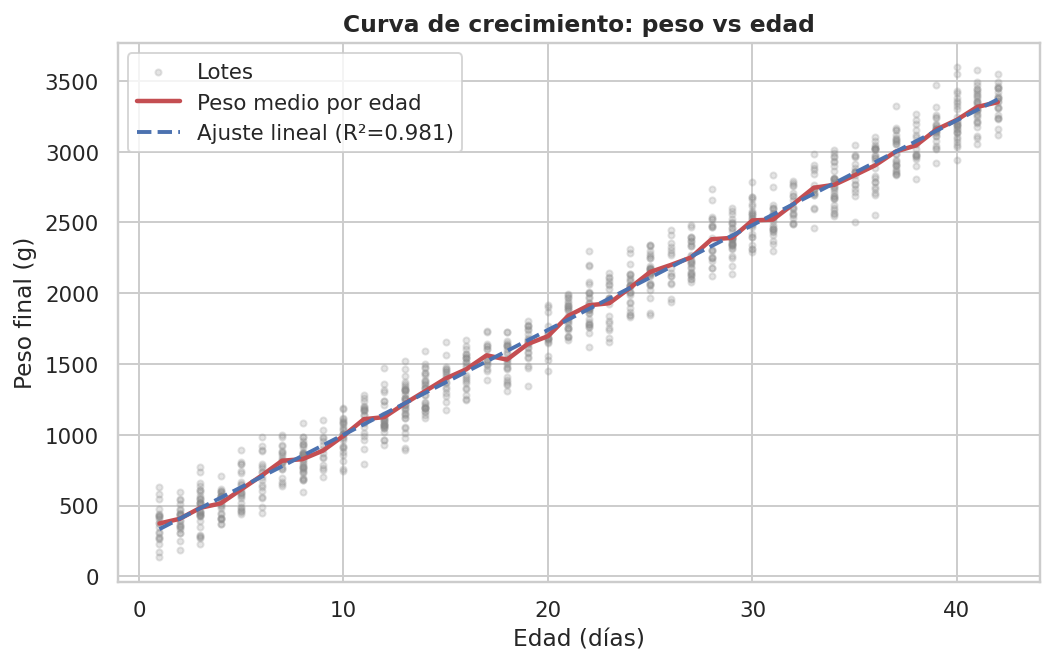
\includegraphics[width=0.86\linewidth]{01_curva_crecimiento.png}
\caption{Curva de crecimiento: peso final frente a edad, con ajuste lineal. El crecimiento es
prácticamente recto en el rango 1--42 días.}
\label{fig:curva}
\end{figure}

\subsection{Estructura de correlación e información}
El mapa de correlaciones (Figura~\ref{fig:corr}) confirma que \textbf{edad} ($r = 0{,}99$) y
\textbf{consumo de alimento} ($r = 0{,}96$) dominan la relación con el peso, pero también que ambas están
fuertemente correlacionadas entre sí ($r = 0{,}95$): aportan información en buena medida redundante. Las
variables ambientales muestran correlación $\approx 0$ con el objetivo.

\begin{figure}[H]
\centering
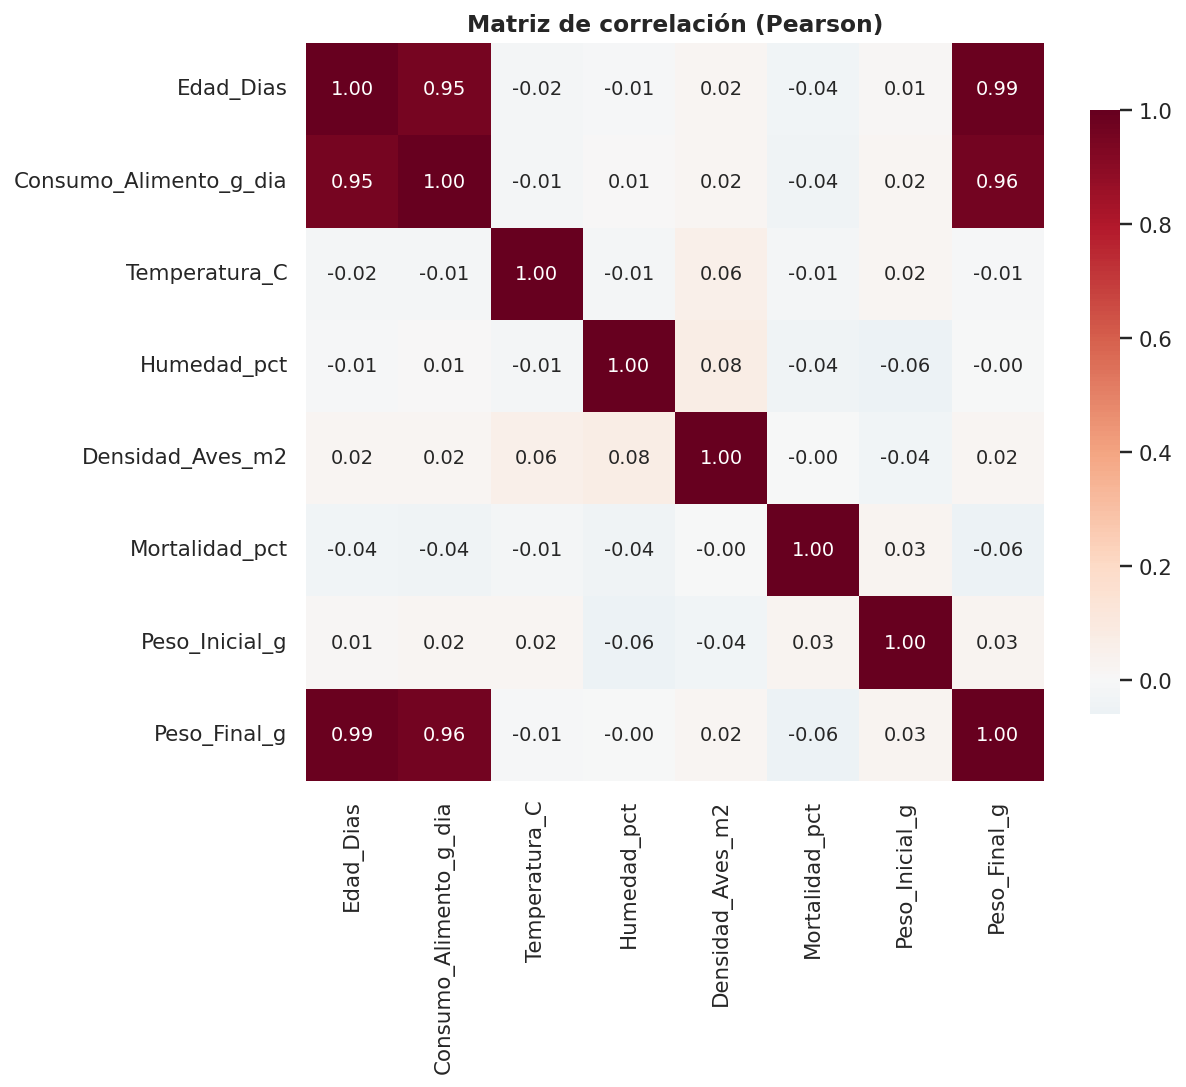
\includegraphics[width=0.82\linewidth]{02_correlacion.png}
\caption{Matriz de correlación de Pearson entre variables numéricas y el objetivo.}
\label{fig:corr}
\end{figure}

Para no quedarnos solo con relaciones lineales, se calculó la \textbf{información mutua} (Figura~\ref{fig:mi}),
que captura dependencias de cualquier forma. El resultado es contundente y a la vez revelador:

\begin{figure}[H]
\centering
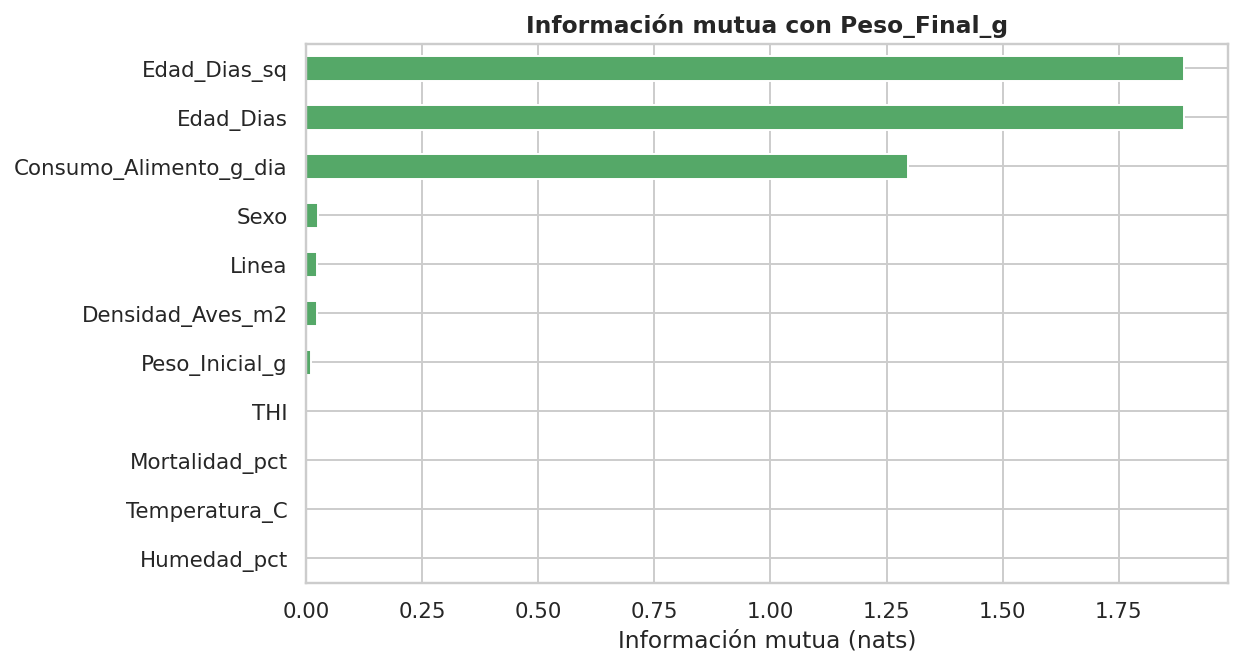
\includegraphics[width=0.78\linewidth]{05_mutual_info.png}
\caption{Información mutua de cada variable con el peso final. Edad y consumo concentran la señal;
temperatura, humedad y mortalidad aportan prácticamente cero.}
\label{fig:mi}
\end{figure}

\hallazgo{\textbf{Temperatura, humedad y mortalidad tienen información mutua exactamente nula} con el
objetivo: no hay señal ni lineal ni no lineal. Esto contradice la biología conocida (el estrés térmico
afecta el engorde), por lo que se interpreta como un \textbf{problema de calidad/registro del dato}, no
como evidencia de que el ambiente sea irrelevante. La recomendación operativa es reforzar la sensórica
y el registro ambiental por galpón.}

\subsection{Distribuciones y dispersión por grupos}
Las distribuciones de las variables clave (Figura~\ref{fig:dist}) son regulares y sin colas anómalas. El
diagrama de dispersión edad--peso segmentado por sexo y línea (Figura~\ref{fig:scatter}) muestra
visualmente lo que después confirma el modelo: los machos se sitúan por encima de las hembras y Cobb~500
encabeza la nube de puntos en la zona de faena.

\begin{figure}[H]
\centering
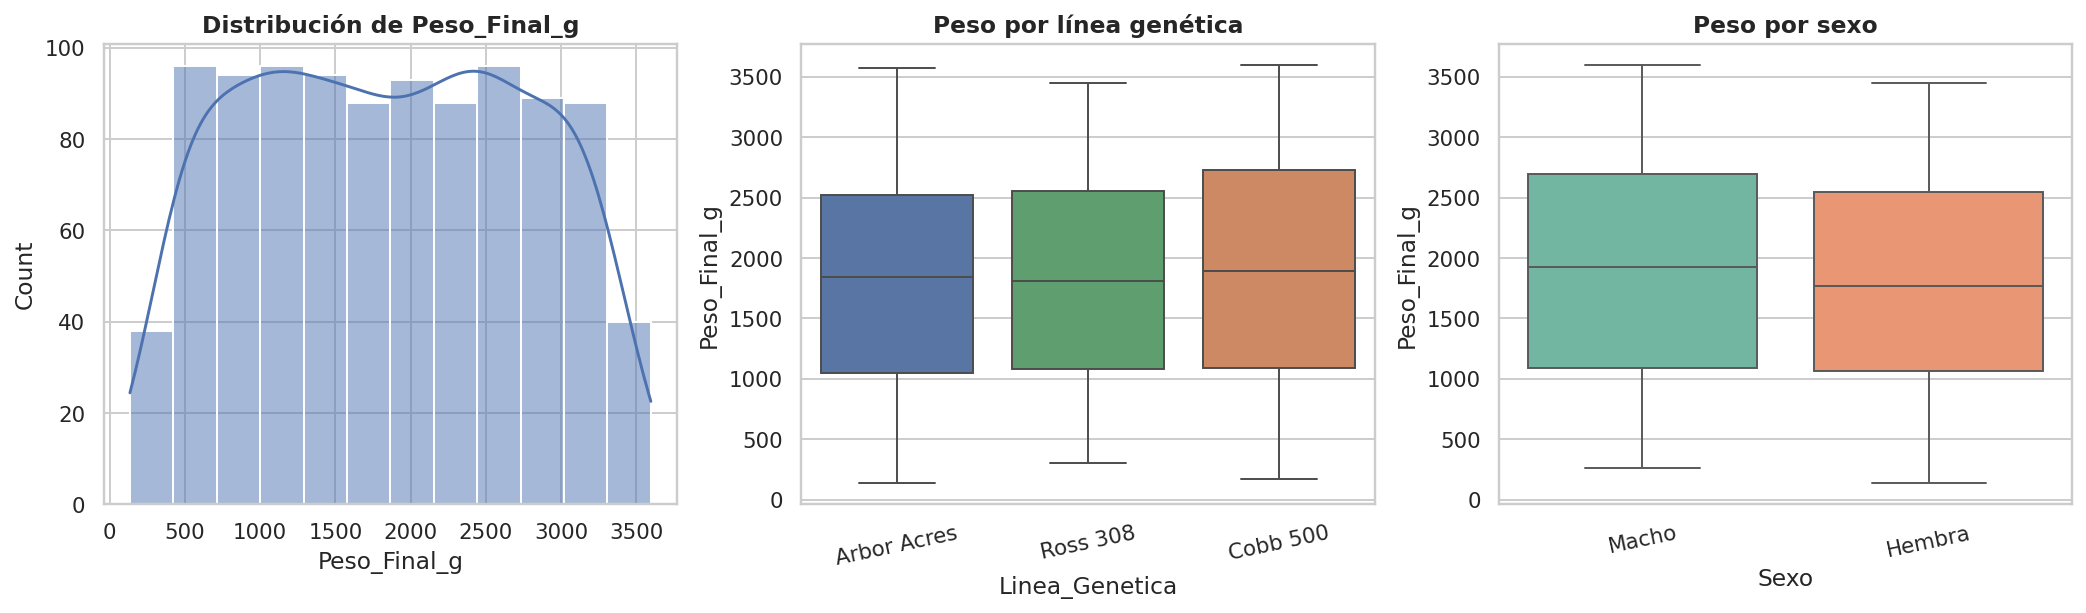
\includegraphics[width=0.95\linewidth]{03_distribuciones.png}
\caption{Distribuciones de las principales variables numéricas.}
\label{fig:dist}
\end{figure}

\begin{figure}[H]
\centering
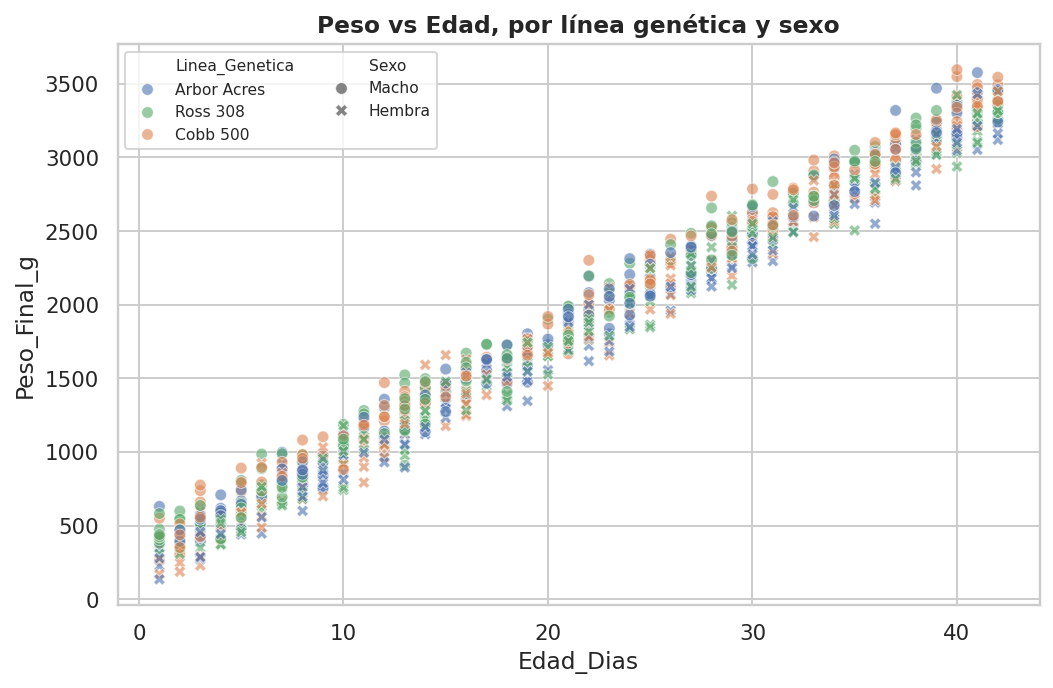
\includegraphics[width=0.95\linewidth]{04_scatter_edad_peso.png}
\caption{Peso final frente a edad, diferenciado por sexo y por línea genética.}
\label{fig:scatter}
\end{figure}

\subsection{Análisis de componentes principales (PCA)}
El PCA (Figura~\ref{fig:pca}) resume la geometría del problema: las dos primeras componentes capturan la
mayor parte de la varianza, y el \emph{biplot} muestra los vectores de edad y consumo casi superpuestos
(redundancia) y apuntando en la dirección de máximo peso. El PCA aquí cumple un rol \textbf{diagnóstico}
—evidenciar colinealidad y la dimensionalidad efectiva del problema— más que de reducción para el modelo
final.

\begin{figure}[H]
\centering
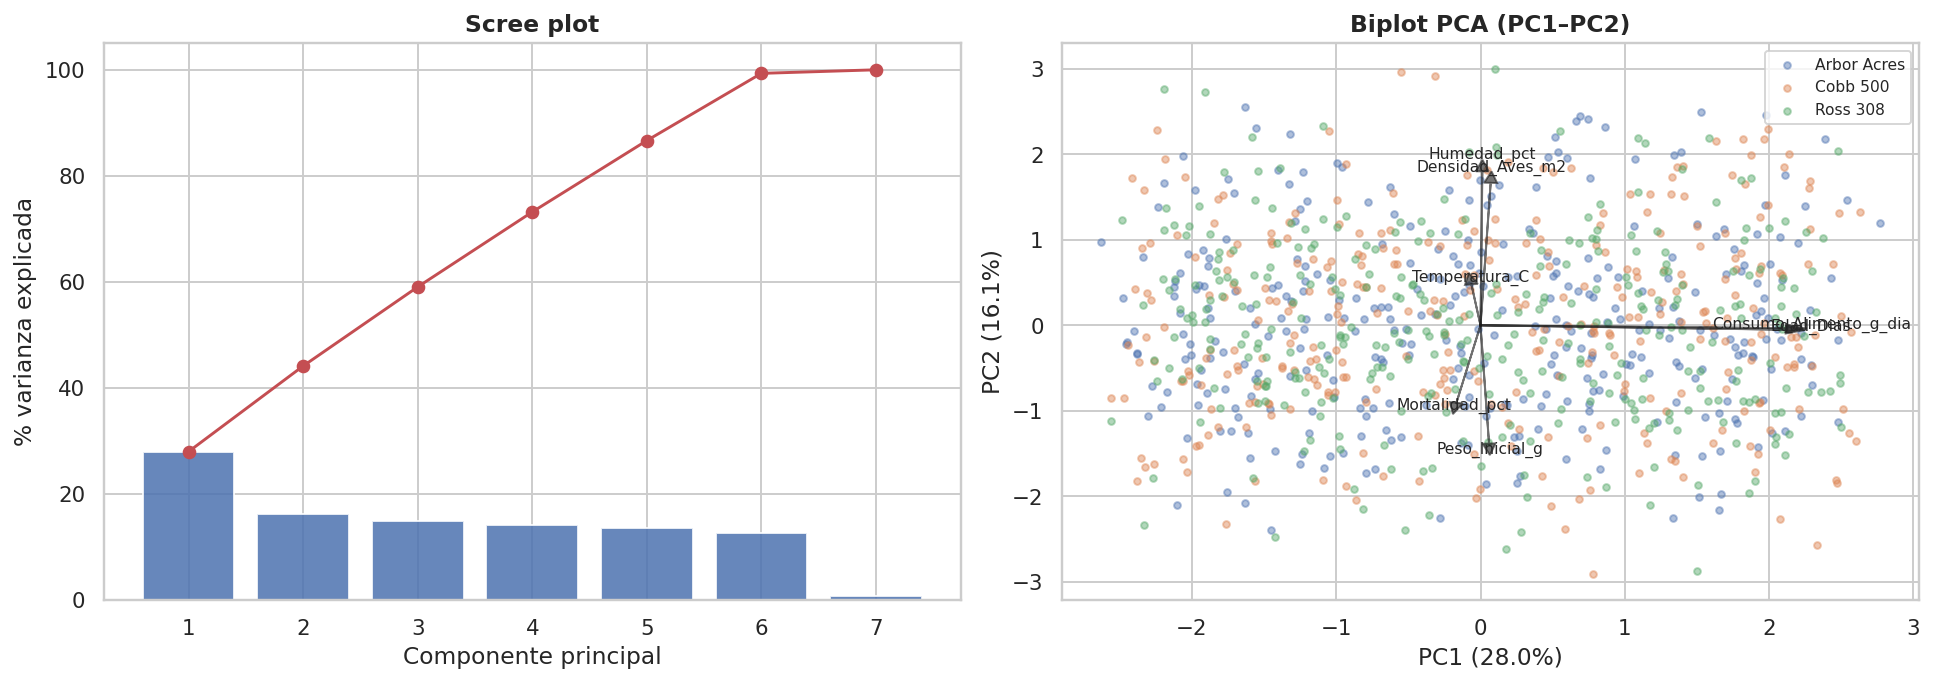
\includegraphics[width=0.95\linewidth]{06_pca.png}
\caption{PCA: varianza explicada acumulada y \emph{biplot} de cargas sobre las dos primeras componentes.}
\label{fig:pca}
\end{figure}

% =========================================================================
% 5. SELECCIÓN DE VARIABLES
% =========================================================================
\section{Selección de variables}
\label{sec:seleccion}

\subsection{Control de fuga de información (\emph{data leakage})}
Este es el punto metodológico más delicado del caso y donde se concentra el criterio \emph{senior}.
Variables como la \textbf{ganancia de peso}, la \textbf{ganancia diaria (GDP)} o el
\textbf{índice de conversión alimenticia (FCR)} se derivan directamente del peso final. Usarlas como
predictoras produciría un modelo con métricas espectaculares pero \textbf{inútil en producción}, porque
en el momento de predecir todavía no se conoce el peso final. Por ello se aislaron en un objeto de
\emph{descriptores de negocio} y \textbf{nunca} entraron al modelo. Solo se usaron como lectura
económica a posteriori.

\subsection{Variables seguras y su capacidad incremental}
El conjunto de predictoras seguras quedó en: numéricas \{Edad, Consumo, Temperatura, Humedad, Densidad,
Mortalidad, Peso\_Inicial, Edad$^2$, THI\} y categóricas \{Sexo, Línea genética\}. Para cuantificar
\emph{cuánto aporta cada bloque} se midió el $R^2$ de validación cruzada al ir añadiendo variables de
forma acumulada (Figura~\ref{fig:capacidad} y Tabla~\ref{tab:capacidad}).

\begin{figure}[H]
\centering
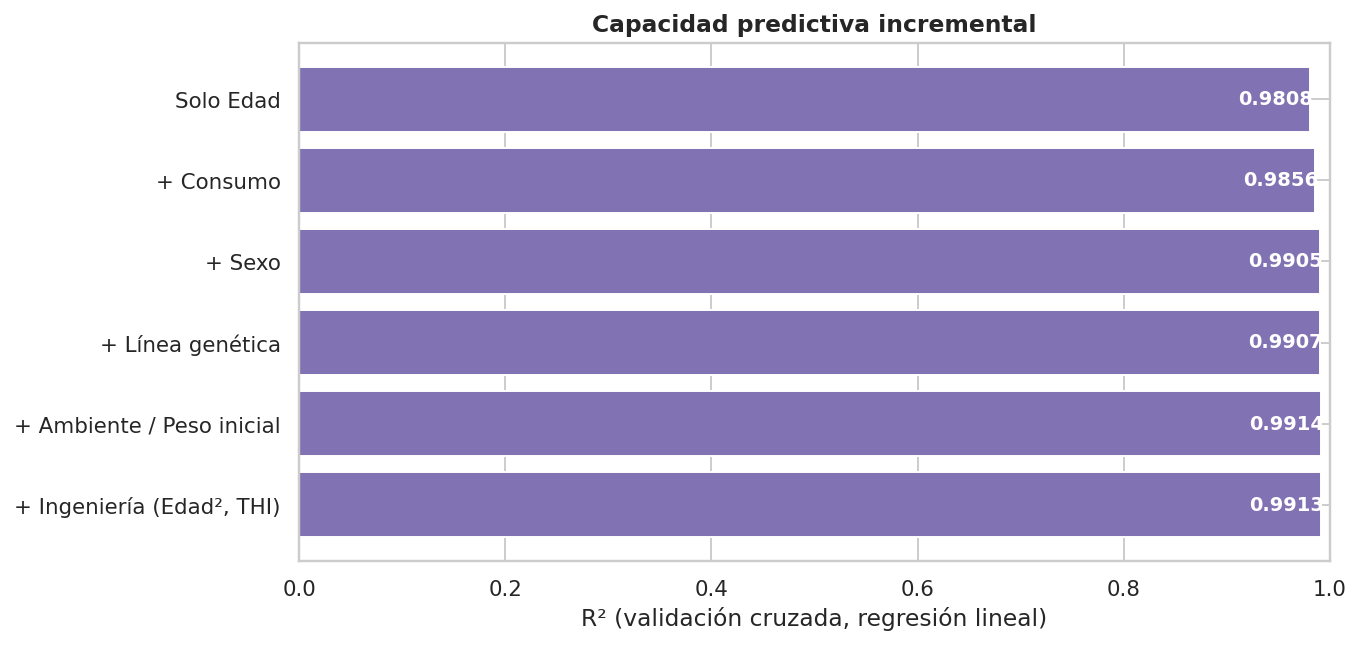
\includegraphics[width=0.8\linewidth]{07_capacidad_incremental.png}
\caption{Capacidad predictiva incremental ($R^2$ en validación cruzada) al añadir bloques de variables.}
\label{fig:capacidad}
\end{figure}

\begin{table}[H]
\centering
\caption{Capacidad predictiva incremental por bloque de variables.}
\label{tab:capacidad}
\small
\begin{tabular}{l S[table-format=1.4]}
\toprule
\textbf{Conjunto de variables} & {\textbf{$R^2$ (CV)}}\\
\midrule
Solo Edad                          & 0.9808\\
\quad + Consumo                    & 0.9856\\
\quad + Sexo                       & 0.9905\\
\quad + Línea genética             & 0.9907\\
\quad + Ambiente / Peso inicial    & 0.9914\\
\quad + Ingeniería (Edad$^2$, THI) & 0.9913\\
\bottomrule
\end{tabular}
\end{table}

\hallazgo{La edad sola ya alcanza $R^2 = 0{,}981$. El \textbf{segundo factor más rentable es el sexo}
(salto a $0{,}990$), por encima de la línea genética. El ambiente y la ingeniería de variables aportan
mejoras marginales o nulas, coherente con el carácter lineal y sintético del dato. \textbf{Esto justifica
preferir un modelo lineal y parsimonioso.}}

% =========================================================================
% 6. MODELADO Y COMPARACIÓN
% =========================================================================
\section{Modelado y comparación de métricas}

\subsection{Diseño experimental}
Se aplicó una partición \textbf{80/20 estratificada por quintiles de edad} para que train y test cubran
todo el ciclo de cría. El preprocesamiento se encapsuló en un \texttt{ColumnTransformer} dentro de un
\texttt{Pipeline} (imputación + estandarización para numéricas; imputación + \emph{one-hot} con
\texttt{drop='first'} para categóricas), evitando cualquier fuga del conjunto de prueba. La comparación
se hizo con \textbf{validación cruzada de 5 particiones} usando el RMSE como criterio.

\subsection{Banco de modelos y resultados}
Se evaluaron once modelos, desde un \emph{baseline} trivial (predecir la media) hasta \emph{gradient
boosting}. La Tabla~\ref{tab:modelos} y la Figura~\ref{fig:modelos} resumen el desempeño.

\begin{table}[H]
\centering
\caption{Comparación de modelos por validación cruzada (5 particiones), ordenados por RMSE.}
\label{tab:modelos}
\small
\begin{tabular}{l S[table-format=3.2] S[table-format=2.2] S[table-format=3.2] S[table-format=1.4]}
\toprule
\textbf{Modelo} & {\textbf{RMSE (g)}} & {\textbf{$\pm$ sd}} & {\textbf{MAE (g)}} & {\textbf{$R^2$ (CV)}}\\
\midrule
\rowcolor{grisclaro}
Lasso (campeón)        & 85.16  & 3.04 & 68.09  & 0.9910\\
Regresión Lineal       & 85.19  & 3.04 & 68.11  & 0.9910\\
Ridge                  & 85.34  & 3.13 & 68.28  & 0.9910\\
ElasticNet             & 86.52  & 3.20 & 69.47  & 0.9907\\
Gradient Boosting      & 89.70  & 2.49 & 71.16  & 0.9900\\
XGBoost                & 92.62  & 3.13 & 73.80  & 0.9893\\
LightGBM               & 93.12  & 3.74 & 74.59  & 0.9892\\
Random Forest          & 104.04 & 4.99 & 81.98  & 0.9865\\
SVR (RBF)              & 145.13 & 7.13 & 109.95 & 0.9738\\
KNN ($k=10$)           & 193.72 & 6.88 & 155.14 & 0.9536\\
Baseline (media)       & 902.80 & 26.33 & 783.06 & -0.0059\\
\bottomrule
\end{tabular}
\end{table}

\begin{figure}[H]
\centering
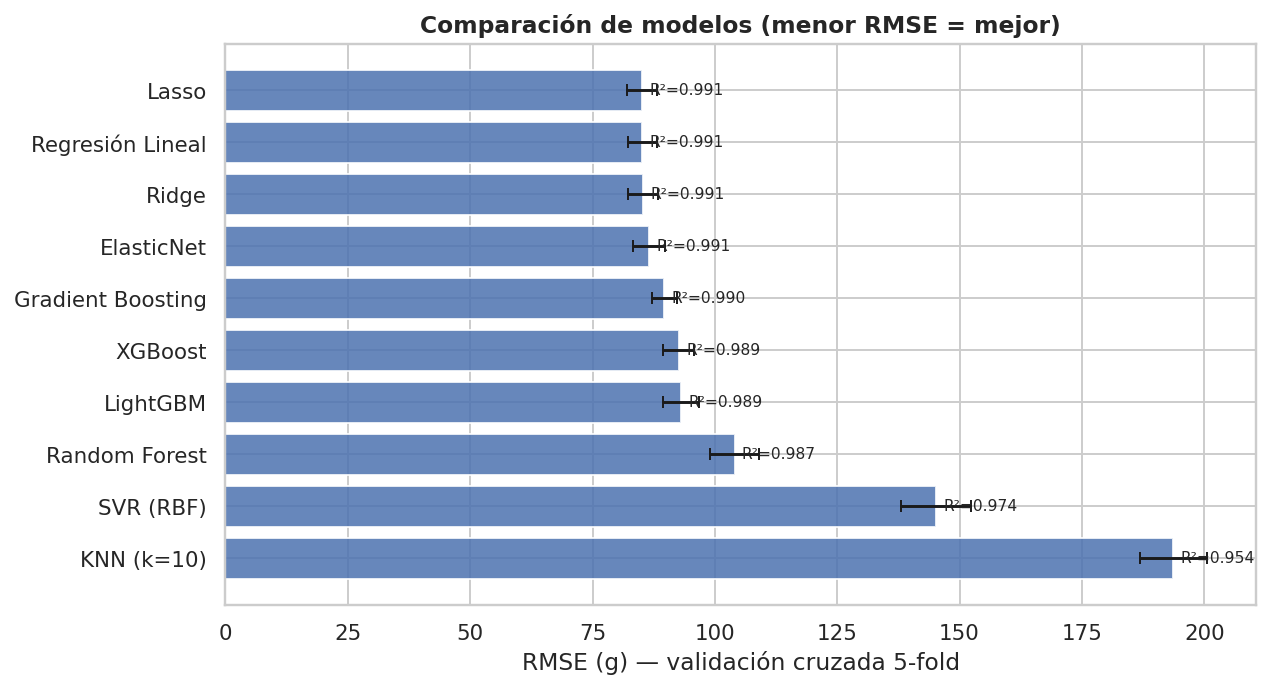
\includegraphics[width=0.9\linewidth]{08_comparacion_modelos.png}
\caption{RMSE en validación cruzada por modelo (menor es mejor). La familia lineal lidera.}
\label{fig:modelos}
\end{figure}

\subsection{Modelo campeón y principio de parsimonia}
Los cuatro mejores modelos son lineales y están prácticamente empatados (RMSE entre \num{85.2} y
\num{86.5}\,\si{\gram}). Los métodos de árboles, pese a su flexibilidad, \textbf{no superan} a la regresión
y muestran mayor varianza. Ante un empate técnico, se eligió la \textbf{regresión Lasso} por su
simplicidad, su capacidad de regularización (puede llevar coeficientes irrelevantes a cero, reforzando la
interpretabilidad) y su facilidad de despliegue y mantenimiento.

\medskip
\noindent\textbf{Desempeño del campeón sobre el conjunto de prueba (datos no vistos):}

\begin{table}[H]
\centering
\caption{Métricas finales del modelo Lasso sobre el conjunto de prueba (20\%).}
\label{tab:campeon}
\small
\begin{tabular}{l S[table-format=2.4]}
\toprule
\textbf{Métrica} & {\textbf{Valor}}\\
\midrule
RMSE (g) & 83.08\\
MAE (g)  & 64.58\\
$R^2$    & 0.9921\\
MAPE (\%)& 5.82\\
\bottomrule
\end{tabular}
\end{table}

El diagnóstico de residuos (Figura~\ref{fig:diag}) confirma un buen ajuste: los predichos siguen la
diagonal frente a los observados y los residuos se reparten sin estructura evidente alrededor de cero.

\begin{figure}[H]
\centering
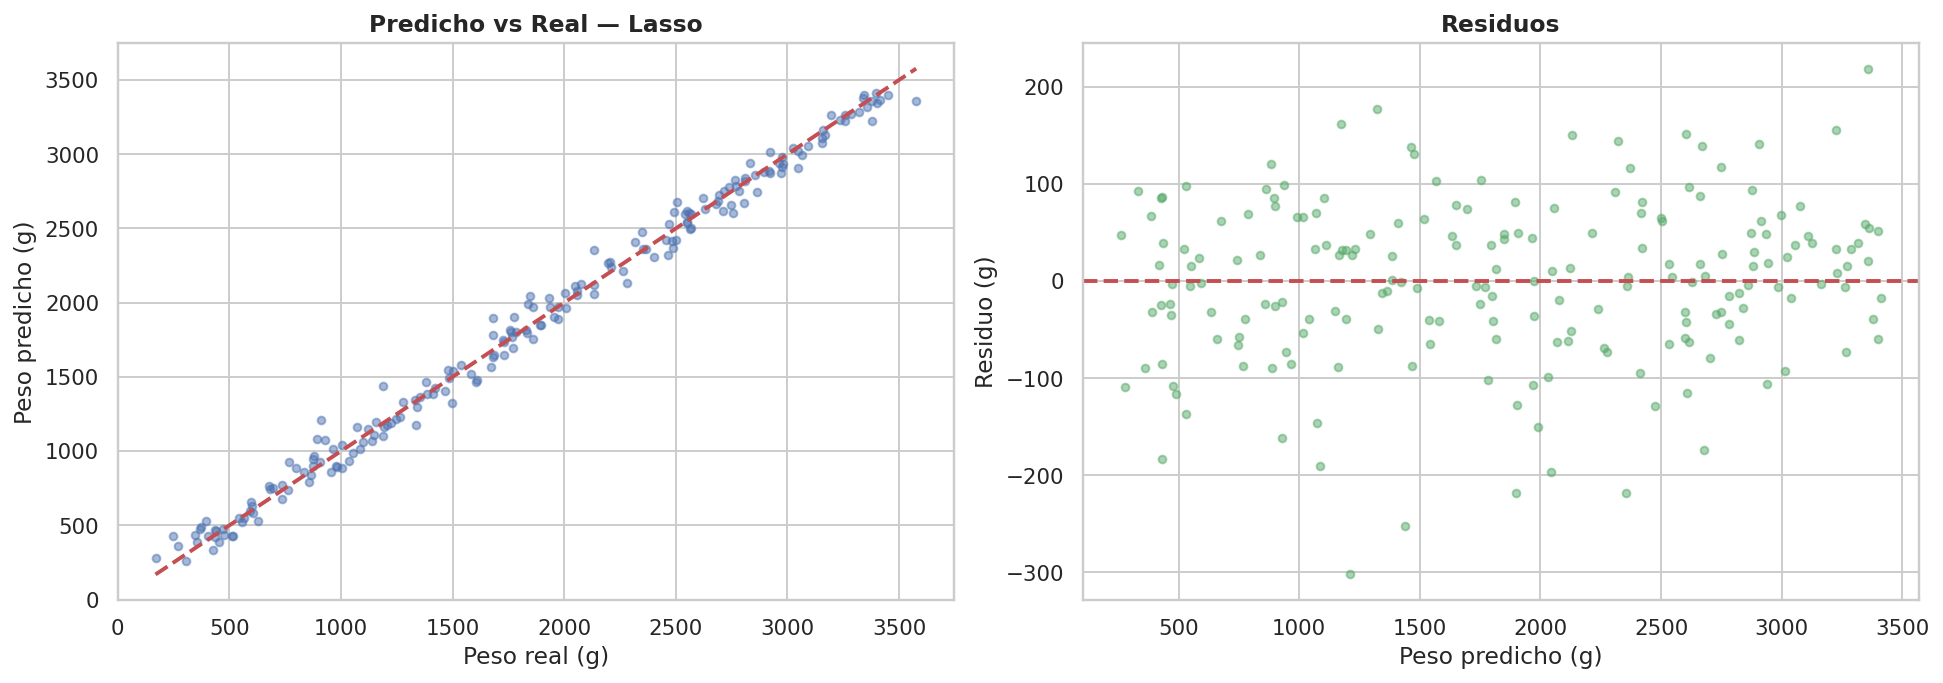
\includegraphics[width=0.95\linewidth]{09_diagnostico_campeon.png}
\caption{Diagnóstico del modelo campeón: valores predichos frente a observados y análisis de residuos.}
\label{fig:diag}
\end{figure}

% =========================================================================
% 7. IMPORTANCIA Y HALLAZGOS DE NEGOCIO
% =========================================================================
\section{Importancia de variables y hallazgos de negocio}

\subsection{Importancia por permutación}
Para una lectura \emph{agnóstica al modelo}, se calculó la importancia por permutación sobre el conjunto
de prueba (Figura~\ref{fig:imp}). El resultado es consistente con todo lo anterior: \textbf{la edad es,
con diferencia, la variable más determinante}, seguida del consumo de alimento; el sexo aparece como el
factor categórico de mayor peso.

\begin{figure}[H]
\centering
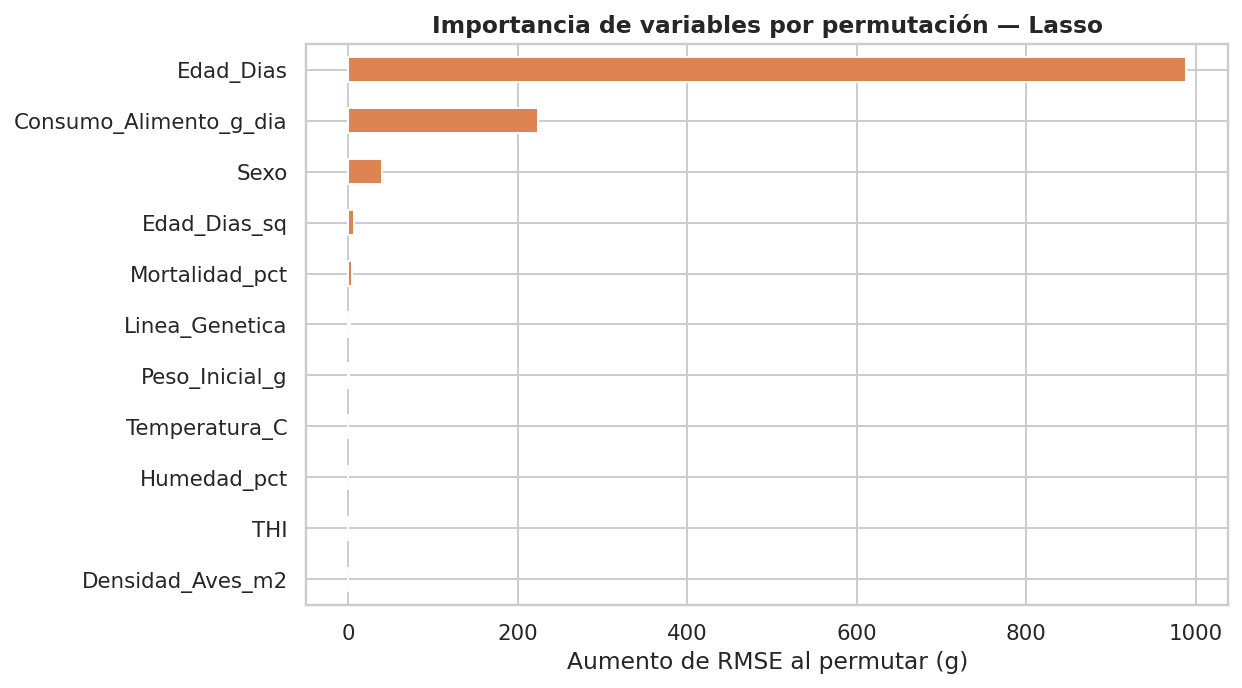
\includegraphics[width=0.8\linewidth]{10_importancia.png}
\caption{Importancia de variables por permutación (caída del desempeño al permutar cada variable).}
\label{fig:imp}
\end{figure}

\subsection{Efecto ajustado de la línea genética}
Comparar el peso medio crudo por línea sería engañoso, porque las líneas podrían no estar igualmente
distribuidas en edad y sexo. Por eso se estimó el \textbf{efecto ajustado} mediante una regresión
(MCO/\emph{OLS}) que controla edad y sexo ($R^2 = 0{,}986$), reportando intervalos de confianza al
95\,\% (Tabla~\ref{tab:efectos}). Esta es la forma correcta y auditable de responder ``¿qué línea
engorda más?''.

\begin{table}[H]
\centering
\caption{Efecto ajustado sobre el peso final (g), controlando edad y sexo. Categorías base: Arbor Acres y Hembra.}
\label{tab:efectos}
\small
\begin{tabular}{l S[table-format=3.1] S[table-format=3.1] S[table-format=3.1]}
\toprule
\textbf{Factor} & {\textbf{Efecto (g)}} & {\textbf{IC 95\% inf.}} & {\textbf{IC 95\% sup.}}\\
\midrule
Sexo: Macho                 & 126.4 & 113.2 & 139.7\\
Línea: Cobb 500             & 44.3  & 28.1  & 60.5\\
Línea: Ross 308             & 25.2  & 9.1   & 41.4\\
\bottomrule
\end{tabular}
\end{table}

\hallazgo{\textbf{Cobb 500 es la línea que más engorda} (\SI{+44.3}{\gram} sobre Arbor Acres, ajustado),
seguida de Ross 308 (\SI{+25.2}{\gram}). Ambos efectos son significativos (sus IC no cruzan cero). Sin
embargo, el \textbf{efecto del sexo (\SI{+126.4}{\gram}) casi triplica al de la mejor línea}: la estrategia
de sexado y manejo diferenciado por sexo es, en peso, más palanca que la elección de línea.}

\subsection{Peso a faena y consumo por línea}
Mirando solo lotes próximos a faena ($\geq 35$ días), el peso medio observado ordena a las líneas igual
que el efecto ajustado, con un consumo de alimento por día muy similar entre ellas
(Tabla~\ref{tab:faena}). Es decir, Cobb~500 logra más peso \emph{sin} un consumo diario marcadamente mayor.

\begin{table}[H]
\centering
\caption{Peso a faena ($\geq 35$ días) y consumo medio por línea genética.}
\label{tab:faena}
\small
\begin{tabular}{l S[table-format=4.0] S[table-format=3.2] c}
\toprule
\textbf{Línea} & {\textbf{Peso medio (g)}} & {\textbf{Consumo (g/día)}} & \textbf{$n$ lotes}\\
\midrule
\rowcolor{grisclaro}
Cobb 500    & 3172 & 190.68 & 66\\
Ross 308    & 3097 & 188.42 & 60\\
Arbor Acres & 3082 & 184.88 & 62\\
\bottomrule
\end{tabular}
\end{table}

\subsection{Traducción económica (monetización auditable)}
Para convertir gramos en dólares se usaron referencias \textbf{públicas y verificables} del mercado
ecuatoriano (ver Sección~\ref{sec:refs}): precio del pollo en pie de referencia \SI{1.65}{USD\per\kilo}
(rango de sensibilidad \SIrange{1.45}{1.85}{USD\per\kilo}). Bajo este supuesto y un lote tipo de
\num{10000} aves, el diferencial de peso de Cobb~500 frente a Arbor Acres se traduce en del orden de
\textbf{\SI{1481}{USD} de ingreso bruto adicional por lote}; Ross~308 aporta unos \SI{254}{USD} por lote
(Tabla~\ref{tab:dinero}). Es una estimación de \emph{ingreso} por mayor peso; el margen neto dependería
del costo del balanceado (referencia maíz amarillo $\approx$ \SI{0.428}{USD\per\kilo}) y del FCR real de
cada línea.

\begin{table}[H]
\centering
\caption{Impacto económico estimado por lote de \num{10000} aves (precio en pie \SI{1.65}{USD\per\kilo}).}
\label{tab:dinero}
\small
\begin{tabular}{l S[table-format=1.3] S[table-format=1.3] S[table-format=4.0]}
\toprule
\textbf{Línea} & {\textbf{Peso (kg)}} & {\textbf{$\Delta$kg vs base}} & {\textbf{$\Delta$USD/lote}}\\
\midrule
\rowcolor{grisclaro}
Cobb 500    & 3.172 & 0.090 & 1481\\
Ross 308    & 3.097 & 0.015 & 254\\
Arbor Acres & 3.082 & 0.000 & 0\\
\bottomrule
\end{tabular}
\end{table}

\subsection{Sobre el FCR (conversión alimenticia)}
El dataset registra consumo \emph{diario} pero no \emph{acumulado}, por lo que el FCR verdadero
(alimento total / ganancia total) no es computable de forma exacta. El consumo diario similar entre
líneas (Tabla~\ref{tab:faena}) sugiere que Cobb~500 convierte al menos tan bien como las demás, pero
\textbf{esta conclusión queda pendiente de validación} con consumo acumulado por fase.

% =========================================================================
% 8. CONCLUSIONES
% =========================================================================
\section{Conclusiones capitalizables y auditables}

\begin{enumerate}[leftmargin=1.5em,itemsep=4pt]
  \item \textbf{El peso final es altamente predecible.} Con un modelo lineal simple se obtiene
        $R^2 = 0{,}9921$ y un error porcentual medio de apenas \SI{5.82}{\percent} en datos no vistos.
        La planta puede estimar el peso de faena de un lote con buena precisión a partir de variables
        que conoce \emph{antes} de pesar.
  \item \textbf{La edad y el consumo gobiernan el engorde}; el resto de variables ajusta en los márgenes.
        Esto orienta el control operativo hacia el cumplimiento de la curva de crecimiento por edad.
  \item \textbf{Para maximizar peso, la palanca número uno es el sexo} (\SI{+126}{\gram} machos) y la número
        dos es elegir \textbf{Cobb 500} (\SI{+44}{\gram} ajustado), seguida de Ross~308 (\SI{+25}{\gram}).
        Ambas conclusiones son estadísticamente sólidas (IC al 95\,\%) y coinciden con la literatura
        para clima tropical.
  \item \textbf{Cobb 500 conviene cuando el objetivo es peso/volumen}, y lo logra con un consumo diario
        comparable al de las otras líneas, lo que la hace la mejor candidata para engorde en el contexto
        ecuatoriano —sujeto a confirmar FCR con datos de consumo acumulado—.
  \item \textbf{Hay dinero medible en la decisión genética:} del orden de \SI{1481}{USD} por lote de
        \num{10000} aves al migrar a Cobb~500 frente a Arbor Acres, solo por mayor peso.
\end{enumerate}

\section{Recomendaciones}

\begin{enumerate}[leftmargin=1.5em,itemsep=4pt]
  \item \textbf{Adoptar Cobb 500 como línea preferente para engorde}, priorizando lotes de machos cuando
        el mercado premie el peso, y monitorear el FCR real para confirmar la ventaja económica.
  \item \textbf{Mejorar la captura de datos ambientales.} La señal nula de temperatura, humedad y
        mortalidad es un problema de medición, no una verdad biológica. Instalar/calibrar sensores por
        galpón y registrar a mayor frecuencia permitirá capitalizar esa información en el modelo.
  \item \textbf{Registrar consumo de alimento acumulado por fase} (iniciador, crecimiento, engorde) para
        habilitar un módulo de FCR y de \emph{margen por lote} automático.
  \item \textbf{Desplegar el modelo lineal} como estimador de peso de faena (es ligero, interpretable y
        auditable) e integrarlo con precios de mercado por fecha para proyectar ingresos por lote.
  \item \textbf{Incorporar marca temporal de lote} para migrar, a futuro, a una validación
        \emph{out-of-time} que simule fielmente el despliegue.
\end{enumerate}

\section{Limitaciones}
\begin{itemize}[leftmargin=1.4em,itemsep=2pt]
  \item \textbf{Dato sintético y lineal:} la relación peso--edad es lineal con intercepto no físico; un
        dataset real (curva de Gompertz) exigiría términos no lineales, ya habilitados en el pipeline
        (\texttt{Edad\_Dias\_sq}).
  \item \textbf{Ambiente sin señal:} probablemente por la forma en que se generaron/registraron los datos;
        no debe leerse como ausencia de efecto biológico.
  \item \textbf{FCR aproximado:} sin consumo acumulado, el índice de conversión real no es calculable.
  \item \textbf{Precios externos:} la monetización usa referencias de mercado auditables, no precios
        internos de la empresa; los valores absolutos deben recalibrarse con datos propios.
\end{itemize}

% =========================================================================
% 9. REFERENCIAS
% =========================================================================
\section{Referencias y fuentes auditables}
\label{sec:refs}

\subsection*{Literatura sobre líneas genéticas (rendimiento comparado)}
\begin{thebibliography}{99}
\setlength{\itemsep}{2pt}

\bibitem{sciencedirect2025} Estudio comparativo de desempeño en pollos de engorde (Cobb~500, Ross~308 y
otras líneas), \emph{ScienceDirect}, 2025. Reporta superioridad de Cobb~500 en peso corporal, ganancia
de peso y conversión alimenticia. Disponible en:
\url{https://www.sciencedirect.com/science/article/pii/S000390982500284X}

\bibitem{ajol} \emph{Animal Research International} (AJOL). Comparación de rendimiento entre líneas
comerciales en clima tropical: Cobb~500 alcanza el mayor peso corporal final frente a Arbor Acre y
Ross~308. Disponible en: \url{https://www.ajol.info/index.php/ari/article/view/239731}

\bibitem{fidar} Comparativa técnica Cobb~500 vs.\ Ross~308 (parámetros productivos y de conversión).
\emph{Fidar Feed}. Disponible en: \url{https://fidarfeed.com/}

\bibitem{thom1959} Thom, E.C. (1959). \emph{The Discomfort Index} (Temperature--Humidity Index, THI).
\emph{Weatherwise}, 12(2), 57--61. Base del índice de estrés térmico empleado en la ingeniería de variables.
\end{thebibliography}

\subsection*{Fuentes de precios — mercado avícola ecuatoriano}
\begin{thebibliography}{99}
\setlength{\itemsep}{2pt}

\bibitem{conave} CONAVE — Corporación Nacional de Avicultores del Ecuador. Estadísticas de precios de
maíz amarillo y mercado avícola (2024--2025). \url{https://www.conave.org/}

\bibitem{expreso} \emph{Diario Expreso} (nov.\ 2025). Reporte de precios del maíz amarillo
($\approx$ \SI{19.40}{USD} por quintal $\equiv$ \SI{428}{USD\per ton} $\equiv$ \SI{0.428}{USD\per\kilo}).
\url{https://www.expreso.ec/}

\bibitem{elproductor} \emph{El Productor}. Costos de producción y precios de venta del pollo en pie en
Ecuador. \url{https://elproductor.com/}

\bibitem{avinews} \emph{aviNews}. Coyuntura de precios y costos del sector avícola.
\url{https://avinews.com/}

\bibitem{pollosec} Portal \emph{Pollos.ec} y \emph{Ecuaquimica}. Referencias de precio del pollo en pie
y de balanceado por saco. \url{https://pollos.ec/} ; \url{https://www.ecuaquimica.com.ec/}
\end{thebibliography}

\vspace{0.5cm}
\noindent\rule{\linewidth}{0.4pt}\\[2pt]
{\footnotesize Todos los resultados numéricos de este informe provienen de la ejecución reproducible del
cuaderno \texttt{pipeline\_pollos.ipynb} (semilla \texttt{42}). Las figuras se generan en
\texttt{outputs/figures/} y las tablas en \texttt{outputs/tablas/}.}

\end{document}
